\documentclass[11pt,a4paper]{article}
\usepackage{fontspec}
% Pagella's book-style serif is paired with matching OpenType mathematics.
\setmainfont{TeX Gyre Pagella}[Ligatures=TeX]
\setsansfont{TeX Gyre Heros}[Scale=MatchLowercase]
\setmonofont{TeX Gyre Cursor}[Scale=MatchLowercase]
\usepackage{microtype,amsmath,mathtools,graphicx,booktabs,longtable,array}
\usepackage[warnings-off={mathtools-colon,mathtools-overbracket}]{unicode-math}
\setmathfont{TeX Gyre Pagella Math}
\usepackage{xcolor,titlesec,fvextra,needspace}
\DefineVerbatimEnvironment{CNSAlgorithm}{Verbatim}{fontsize=\footnotesize,breaklines=true,breakanywhere=true,frame=lines,framesep=3mm}
\definecolor{CNSInk}{HTML}{243446}
\definecolor{CNSBlue}{HTML}{0F4D92}
\definecolor{CNSMuted}{HTML}{526173}
\titleformat{\section}{\large\sffamily\bfseries\color{CNSInk}}{\thesection}{0.75em}{}
\titleformat{\subsection}{\normalsize\sffamily\bfseries\color{CNSInk}}{\thesubsection}{0.75em}{}
\titlespacing*{\section}{0pt}{2.0ex plus .7ex minus .2ex}{1.0ex plus .2ex}
\titlespacing*{\subsection}{0pt}{1.6ex plus .5ex minus .2ex}{0.7ex plus .2ex}
\linespread{1.04}
\clubpenalty=10000
\widowpenalty=10000
\displaywidowpenalty=10000
\usepackage[a4paper,margin=26mm,headheight=14pt,footskip=18pt]{geometry}
\usepackage{enumitem}
\setlist{nosep,leftmargin=*}
\usepackage{float,caption}
\captionsetup{font={small},labelfont={sf,bf},skip=8pt}
\usepackage[section]{placeins}
\usepackage[round]{natbib}
\setcitestyle{numbers,square,sort&compress}
\usepackage{fancyhdr}
\pagestyle{fancy}
\fancyhf{}
\fancyhead[L]{\footnotesize\sffamily\color{CNSMuted} CNS 9.0 · Research proposal · v0.1}
\fancyhead[R]{\footnotesize\sffamily\color{CNSMuted} GTCode.com}
\fancyfoot[C]{\small\sffamily\color{CNSMuted}\thepage}
\renewcommand{\headrulewidth}{0.3pt}
\fancypagestyle{opening}{\fancyhf{}\renewcommand{\headrulewidth}{0pt}\fancyfoot[C]{\small\sffamily\color{CNSMuted}\thepage}}
\usepackage[unicode,pdfencoding=auto,colorlinks=true,linkcolor=CNSBlue,citecolor=CNSBlue,urlcolor=CNSBlue]{hyperref}
\hypersetup{
 pdftitle={Chiral Narrative Synthesis 9.0: Falsification-Guided Narrative Synthesis for Predictive Knowledge Discovery},
 pdfauthor={GTCode.com},
 pdfsubject={Unvalidated research proposal, version 0.1; no CNS 9.0 experiments reported},
 pdfkeywords={CNS 9.0, predictive synthesis, falsification, research proposal},
 pdfcreator={LuaLaTeX / GTCode.com}
}
\urlstyle{same}
\newcommand{\CNSIdentifier}[1]{{\small\ttfamily\def\_{\textunderscore\allowbreak}#1}}
\providecommand{\tightlist}{\setlength{\itemsep}{0pt}\setlength{\parskip}{0pt}}
\emergencystretch=1.2em
\setlength{\parskip}{0.42em}
\setlength{\parindent}{0pt}
% A flush-left title block and full-width abstract replace article's indented
% quotation-style abstract. All layout choices live in this editable source.
\renewenvironment{abstract}{%
  \par\vspace{1.1em}%
  {\sffamily\bfseries\color{CNSInk} Abstract\par}%
  \vspace{0.35em}\small\setlength{\parindent}{0pt}\noindent\ignorespaces
}{\par\vspace{0.9em}\normalsize}
\begin{document}
\thispagestyle{opening}
\begingroup
\raggedright
{\small\sffamily\bfseries\color{CNSBlue} RESEARCH PROPOSAL\enspace /\enspace VERSION 0.1\par}
\vspace{1em}
{\fontsize{27}{31}\selectfont\bfseries Chiral Narrative\newline Synthesis 9.0\par}
\vspace{0.55em}
{\Large Falsification-Guided Narrative Synthesis\par}
\vspace{0.18em}
{\large for Predictive Knowledge Discovery\par}
\vspace{0.9em}
{\normalsize\sffamily GTCode.com\enspace ·\enspace 15 November 2026\par}
\vspace{0.55em}
{\small\sffamily\color{CNSMuted} Conceptual framework · Not empirically evaluated\par}
\endgroup
\vspace{0.8em}
{\color{CNSBlue}\hrule height 0.7pt}
\begin{abstract}
Conflicting accounts can reveal an unrecorded condition, a defective
source, a genuine change in the world, or an irresolvable identification
problem. Existing language-model methods can retrieve supporting
passages, select among answers, or aggregate several responses, but
agreement and internal consistency do not establish that a new
explanation predicts observations beyond the initial record. We propose
\textbf{Chiral Narrative Synthesis 9.0 (CNS 9.0)}, with the working
subtitle \emph{Falsification-Guided Narrative Synthesis}, as a research
framework that turns structured disagreement into bounded explanatory
hypotheses, locked predictions, and permitted observations designed to
distinguish rival accounts. CNS 9.0 inherits Structured Narrative
Objects (SNOs), evidence provenance, and unresolved uncertainty from
earlier CNS proposals; it changes the acceptance test from principally
internal coherence to scoped predictive value and honest evidence-based
revision. Explicit transformation contracts distinguish irrelevant
changes, relevant evidence updates, and genuine changes of the target
phenomenon. We specify the representational objects and an operational
procedure without requiring novel geometric or tensor mathematics. Three
separable research hypotheses concern contrastive reliability,
predictive synthesis, and disagreement-guided evidence acquisition. A
proposed, not preregistered, evaluation proposes ten systems and
planning targets of 2,400 independent confirmatory synthetic scenarios,
with discovery and action subsets, external diagnostics, and prospective
engineering measurements. \textbf{No CNS 9.0 system has been implemented
or experimentally evaluated for this publication.} Its contribution is a
falsifiable research program, not a demonstration that the approach
improves truth-finding.
\end{abstract}

\section{Introduction: when disagreement is
informative}\label{introduction-when-disagreement-is-informative}

Imagine one report stating that enabling a cache reduces request latency
and another reporting that it increases latency. Both statements can be
compatible with reality if request reuse, update frequency, resource
pressure, or freshness constraints differ. They can also be incompatible
because a measurement is faulty, a source copied erroneous numbers, or
one account simply makes a false generalization. The correct response is
not necessarily reconciliation. A system ought to distinguish different
questions, reject unsupported accounts when warranted, and preserve
genuinely unresolved alternatives.

This example exposes a gap between \emph{answer selection} and
\emph{explanatory discovery}. Selecting the more credible report can be
useful. So can identifying the source of a contradiction or expressing
uncertainty. The larger research opportunity is to infer a
\textbf{measurable condition} not stated in either report, state what
new observations that condition predicts, and seek an observation
capable of refuting it. If the condition merely redescribes the evidence
already seen, no discovery has occurred. If the model uses hidden
evaluation labels to invent it, the result is invalid. If a simple
fitted regression does as well, the more elaborate synthesis process has
not justified its cost.

The \emph{Against All Likelihood} essay by Lopez-Paz argues that
language likelihood is neither necessary nor sufficient for objective
truth and explores invariance across relevant transformations as a guide
to more robust knowledge \citep{R01}. That argument motivates testing an
account across contexts, but does not by itself resolve the crucial
question of \textbf{which transformations should preserve which aspect
of an answer}. A stable false statement survives every harmless
paraphrase. A correct account may need to change after a new measurement
or a regime shift. For CNS, this suggests that truth-seeking requires
both robustness to irrelevant differences and correct responsiveness to
relevant differences---not a blanket rule that all answers should agree.

Earlier CNS work proposes synthesizing Structured Narrative Objects,
rather than merely voting on isolated claims. It includes critics,
evidence grounding, access states, bounded invention of additional
predicates, and the possibility of unresolved contradiction
\citep{G02, G03, G11}. CNS 9.0 retains those useful aims while shifting
the scientific burden to new predictions and comparisons with ordinary
alternatives. What matters is not whether the architecture sounds
sophisticated, but whether it improves outcomes that an independent
evaluator can measure.

\textbf{Why begin with narrative disagreement?} Sparse reports can
contain clues about omitted conditions that are absent from a ready-made
table. CNS proposes that comparing opposing accounts can focus a bounded
search over those clues. This is a mechanism hypothesis, especially
relevant when measurements are scarce and candidate moderators are
numerous, not a theorem that prose beats tabular learning. Shared false
assumptions, copied reports or abundant well-measured structured data
may remove the benefit. A common-extractor learner and generic
hypothesis-refinement comparator must receive the same records and
budget; matched contradiction-uninformative packets test whether
disagreement adds value beyond hypothesis generation itself.

\textbf{Scope.} The proposed theory addresses empirical claims with
explicit target variables, accessible records, or feasible observations.
It does not claim a universal criterion of truth, solve disputes of
values, or recover causal structure without identification assumptions.
We propose a concrete representation, a bounded discovery loop, and an
evaluation whose failure would count against central CNS 9.0 claims. No
experimental findings are offered here.

\section{Related work and contribution
boundary}\label{related-work-and-contribution-boundary}

\subsection{Invariance: useful precedent and real
limits}\label{invariance-useful-precedent-and-real-limits}

Invariant causal prediction studies stable relationships under
environmental changes subject to explicit assumptions about the causal
system \citep{R03}. Invariant Risk Minimization (IRM) proposes a
representation in which the same predictor is optimal across training
environments \citep{R02}. These precedents motivate the question,
``Which relationship remains useful under which changes?'' They do
\textbf{not} show that passing prompt-paraphrase tests establishes world
truth, or that the prompt context generated by a language model is
equivalent to an observed intervention. Negative analyses of IRM and
comparisons with tuned empirical-risk baselines are central warnings
against treating invariance as a solved optimization problem
\citep{R04, R05, R06}. Work on discovering environments adds possible
future tools but not a reliable admissibility oracle \citep{R07}.

Lopez-Paz motivates the joint investigation of explanations and
admissible transformations, including the use of new predictions and
attempted falsification \citep{R01}. CNS 9.0 adopts that motivation; it
does not claim these principles as original contributions. His
inference-time sketch generates answers under varied contexts and
extracts an invariant core. CNS 9.0 proposes a different operational
procedure: retain competing scoped explanations, commit their
distinguishing predictions before acquiring outcomes, and select
evidence-gathering actions using a specified rival-separation rule.
Explicit provenance, transformation contracts, and failure states make
that procedure inspectable. Whether this combination improves predictive
synthesis or investigation over simpler alternatives remains an
empirical question.

Behavioral testing supplies a practical precedent for structured
perturbations, and counterfactually augmented examples distinguish
robust behavior from sensitivity to superficial cues \citep{R08, R09}.
However, a transformation that removes the only relevant source is not a
mere nuisance. Neither is changing a measured causal input. A benchmark
must state the expected response for each transformation instead of
rewarding identical strings under every condition.

\subsection{Evidence, source dependence, and warranted
assertion}\label{evidence-source-dependence-and-warranted-assertion}

Retrieval-augmented generation and chain-of-verification can help
connect an answer to accessible evidence \citep{R11, R16}. Source
dependence is a separate issue: many reports may reproduce the same
originating record and therefore should not be treated as independent
confirmations \citep{R10}. This is particularly important when a
seemingly broad consensus is produced by copying. CNS 9.0 distinguishes
(i) whether two claims address the same estimand, (ii) whether they rely
on the same record, and (iii) whether nominally distinct sources share a
lineage. These are not interchangeable quantities.

A cited source can establish that a statement \textbf{was reported}, not
that the statement is automatically correct. Likewise, a valid deduction
from premises remains conditional on the premises. SNOs therefore
preserve exact source spans, time, access and dependency, while a
separate warrant field records whether the claim is source-reported,
derived given premises, empirically supported within scope, refuted
within scope, or unresolved. Existing CNS 8.0 material recognizes the
distinction between an internally stable orthesis and metaphysical
truth; our proposal makes predictive and observation-based tests
additional explicit gates, not a retrospective claim that the prior work
ignored uncertainty \citep{G02, G03, G08}.

\subsection{Aggregation, debate, abduction, and
argumentation}\label{aggregation-debate-abduction-and-argumentation}

Self-consistency aggregates multiple reasoning samples; debate
structures disagreement between models; verification asks targeted
subquestions \citep{R12, R13, R16}. Results of multi-agent comparisons
suggest that debate must be compared against simpler voting or
aggregation rather than credited with improvement by default
\citep{R14}. Model-generated reasons can also be unfaithful to the
causes of a model's answer \citep{R18}, so CNS 9.0 audits short,
externally checkable justifications rather than treating hidden
reasoning traces as evidence.

The distinction between supporting and attacking arguments has a long
formal tradition in abstract argumentation \citep{R32}. Abductive
inference generates candidate explanations from observations;
computational forms include cost-based first-order abduction
\citep{R33}. Inductive logic programming (ILP) supplies a precedent for
bounded, explicit rule and predicate learning \citep{R21}. These
traditions already cover substantial ground claimed informally by many
``discovery'' systems. CNS 9.0 does not claim to invent abduction,
argument attacks, or predicate invention. The proposed contribution is a
specified architecture and evaluation design for
\textbf{contradiction-guided predictive synthesis}. Its research claim
concerns the incremental value of combining these components, rather
than the invention of invariance testing, abductive explanation, or
experimental design individually. The specification alone does not
establish novelty; comparisons with existing hypothesis-generation and
discovery systems must establish what, if anything, the combination
adds.

Iterative hypothesis generation is already a close precedent. HypoGeniC
updates a bank of natural-language hypotheses using prediction errors on
labeled examples \citep{R37}. Qiu and colleagues propose, select and
refine rules with symbolic interpretation, distinguishing rule induction
from reliable application \citep{R38}. These methods motivate a required
refinement comparator, rather than treating discovery as a comparison
only with answer aggregation. Causal Modelling Agents combine LLM
metadata reasoning with data-driven structural causal models
\citep{R39}; that is relevant hybrid causal-modeling precedent, not
evidence for the present CNS composition or a universal intervention
capability.

\subsection{Choosing observations and existing discovery
agents}\label{choosing-observations-and-existing-discovery-agents}

Bayesian experimental design gives a principled account of selecting
actions to reduce uncertainty when the relevant hypotheses, likelihoods
and priors can be specified \citep{R20}. Active learning for causal
structure makes the experimental-choice problem concrete \citep{R31}.
CNS proposes a contrasting heuristic when probability models are
underspecified, but must label that heuristic honestly and compare it
with relevance-only or random acquisition. Nor may success at predicting
under intervention be presented automatically as identification of a
causal graph.

Modern work already explores agentic scientific workflows: \emph{The AI
Scientist} automates parts of idea generation, experimental code and
reporting \citep{R34}; \emph{Co-Scientist} develops scientific
hypotheses through agent coordination and evaluation \citep{R35}; and
\emph{Robin} connects literature agents, analysis and experimental
biology \citep{R36}. These contributions sharply constrain any claim
that CNS invented multiagent research, hypothesis generation or
experiment planning. CNS 9.0 instead proposes to test whether
\textbf{specific contradiction-derived scope rules, prediction
commitments and measured falsification opportunities} add value over
well-resourced alternatives. DiscoveryBench provides a separate transfer
diagnostic, while FEVER, SciFact and AVeriTeC test forms of
source-grounded verification rather than universal truth
\citep{R25, R26, R27, R28}.

\section{Epistemic commitments and
nonclaims}\label{epistemic-commitments-and-nonclaims}

Four distinctions govern the proposal.

\textbf{Truth is not identical to current warrant.} Whether a scoped
proposition is true in the world is separate from whether the available
record supports saying so. The system can update warrant after evidence
arrives without changing the historical fact being described. A true
claim with inaccessible support remains unwarranted; a previously strong
citation can later be retracted.

\textbf{Coherence is not correctness.} Propositions can agree because
they share a mistaken assumption, training artifact or copied source. A
stable internal model can be a sensible computational stopping
condition, not proof of objective truth. This applies to deductive
closure, round-trip translation, majority vote, and invariance over
model-generated perspectives.

\textbf{Stable mechanism is not constant output.} A representation-only
nuisance change should preserve the relevant meaning, up to an explicit
transformation of units or format. If the population, intervention or
measurement changes, a credible explanation may predict a
\emph{different} outcome. If a unique support record disappears, the
empirical event need not change but the warrant may weaken. We therefore
use transformation-specific output relations.

\textbf{Uncertainty is not lack of access.} Observation noise,
unavailable records, open-world ambiguity, and observationally
equivalent mechanisms imply different limitations. Two worlds that
supply exactly the same permitted observations but require different
conclusions cannot be separated merely by more model deliberation. The
legitimate output may be a set of live alternatives and an
identification boundary.

CNS 9.0 treats a proposed new scope condition as a hypothesis until its
operands are observable and it has predictive consequences not exhausted
by the source examples. A cause is not identified merely because a story
explains a correlation. A probabilistic forecast must refer to a
specified event; token likelihood is not used as its substitute. These
commitments are falsifiable at the level of system behavior and
externally measured outcomes; they are not axioms purportedly
guaranteeing truth.

\section{Minimal formal
specification}\label{minimal-formal-specification}

\subsection{Scoped questions, evidence atoms and structured
narratives}\label{scoped-questions-evidence-atoms-and-structured-narratives}

A \textbf{question} is a tuple
\(q=(Y,\mathcal{P},t,\mathcal{I},u,\tau)\): target outcome or
proposition \(Y\), population or workload \(\mathcal{P}\), time/regime
\(t\), intervention or observation context \(\mathcal{I}\), units \(u\),
and decision tolerance \(\tau\). Two reports that use different tuples
need not contradict one another. A question about median latency is not
silently replaced by one about a ninety-ninth percentile.

An \textbf{evidence atom} \(e=(s,z,d,a,\ell,c)\) records a source
identifier \(s\), verifiable text span or measurement \(z\), timestamp
\(d\), access state \(a\), lineage pointer \(\ell\), and
extraction/collection context \(c\). A source-level relation
\(\operatorname{reports}(s,p)\) must never be silently rewritten as
\(p\). A provenance graph may record copying at the span level. Unknown
lineage remains unknown; dependent documents are not deleted merely
because they repeat valid information.

An \textbf{SNO 9}, or Structured Narrative Object, holds a scoped
question, atomic claims with warrant states, their evidence atoms and
source-dependence graph, rival explanatory relations, transformation
contracts, predictions, permissible actions, and a versioned audit
trail. The representation can be JSON or typed records. No manifold,
narrative metric tensor, or topological invariant is required for the
first scientific claim. Earlier CNS structures remain optional
comparators \citep{G02, G09}.

A \textbf{rival} \(h\in\mathcal{H}\) is an explanation with a declared
scope, executable or adjudicable prediction rule where feasible,
constraints, supporting and defeating observations, and a measure of
what is unknown. The rival set includes the possibility that one
original account should be rejected and the possibility that all
available accounts remain insufficient. The bounded generator need not
represent a complete universe of hypotheses.

\subsection{Transformation contracts}\label{transformation-contracts}

Three records must remain separate. A
\textbf{representation/evidence-integrity contract}
\(c_T=(T,\operatorname{pre}_T,r_T,v_T,z_T)\) declares an operation,
preconditions, a property that should be preserved or converted, a
validator and a state
\(z_T\in\{\text{validated},\text{rejected},\text{unknown}\}\). Unit
conversion can require numerical equivariance; a demonstrably redundant
copy must not count as another independent observation. The
preconditions matter: order can encode chronology, a paraphrase can
change scope, and a copied document can contain new evidence. Semantic
validity is not universally decidable by deterministic code. Removing
evidence can change warrant, but does not impose a universal direction
of confidence change.

A \textbf{rival-indexed response commitment} \(r_{T,h}\) states how
hypothesis \(h\) predicts an outcome will respond to a world, regime or
evidence change. Different rivals may make incompatible commitments. The
runtime need not know which mechanism is true before recording that
disagreement. Knowing that an operation preserves units does not
establish that a disputed world change preserves the outcome.

An \textbf{evaluator-only relation} specifies the benchmark's expected
behavior from its sealed state. It scores the method after outputs are
locked and is never passed to runtime as a validated contract.
Gold-admissibility access is a diagnostic ceiling, excluded from
superiority claims.

For a representation/evidence-integrity contract, the check remains
three-valued:

\[
C_T(x)=\begin{cases}
\mathrm{pass},&z_T=\mathrm{validated}\text{ and }r_T\text{ is verified},\\
\mathrm{fail},&z_T=\mathrm{validated}\text{ and }r_T\text{ is violated},\\
\mathrm{unknown},&\text{the contract or necessary evidence is unresolved}.
\end{cases}
\]

For a rival-indexed commitment, the system records predictions and later
adequacy checks, not an oracle verdict about admissibility. Validators,
tolerances and expected evaluation relations must be frozen before
confirmation. A failed or unknown contract cannot be discarded merely
because its result is inconvenient.

\subsection{Bounded scope invention and predictive
commitments}\label{bounded-scope-invention-and-predictive-commitments}

A new scope rule \(g(x;\theta)\) must use publicly measurable variables,
specify units and time, be non-circular, and generate predictions that
differ between at least two live rivals. Initially the rule language
could allow no more than three observed conditions, bounded thresholds
and declared interactions. Four candidate explanations and two rounds of
revision are possible initial engineering caps, not mathematically
privileged constants. An unobserved condition may be proposed for future
measurement, but not asserted as already present.

Before any held-out observation is revealed, the system writes a
\textbf{prediction commitment} \(k=(h,q,\hat y,\tau,a,t_0)\): the
hypothesis, scoped question, predicted value/distribution/direction,
scoring tolerance, evidence action or observation, and timestamp. The
record is hashed or otherwise made immutable. Prediction novelty is
operational: at least one discriminating consequence was not explicitly
stated in the initial accounts and is evaluated on a new observation.
Novelty is not assessed by linguistic surprise or embedding distance.

Ordinary predictive error remains relevant across prespecified
environments:

\[
R_e(M)=\mathbb{E}_{(x,y)\sim P_e}\big[\ell(M(x),y)\big].
\]

Here \(P_e\) is a defined evaluation environment and \(\ell\) is a
task-appropriate loss. If the system outputs a probability for a binary
event, one proper score is Brier loss \((p-y)^2\) \citep{R22}. A
confidence that a \emph{document entails a sentence} is not thereby a
forecast for a \emph{world event}. Report risk alongside coverage, false
promotions, and other hard safeguards rather than conceal failures
inside one weighted eloquence score.

\subsection{Selecting evidence without imaginary
probabilities}\label{selecting-evidence-without-imaginary-probabilities}

The initial proposed acquisition policy is a \textbf{deterministic
set-separation heuristic}. Let \(\mathcal H_c\) be the deduplicated live
candidates with executable commitments on a common outcome, and let
\(A_h(a)\) be candidate \(h\)'s prediction region after the frozen
measurement-noise and decision-tolerance expansion has been applied
exactly once. For feasible actions with strictly positive, declared
costs, define

\[
U(a)=\frac{1}{\operatorname{cost}(a)}
\frac{\displaystyle\sum_{\{h,h'\}\subseteq\mathcal H_c}
\mathbf 1\!\left[A_h(a)\cap A_{h'}(a)=\varnothing\right]}
{\displaystyle\binom{|\mathcal H_c|}{2}},
\qquad a^*=\arg\max_{a\in\mathcal A_{\mathrm{feasible}}}U(a).
\]

This policy is defined only when at least two comparable candidates
exist and every retained candidate supplies an admissible prediction for
the action. Zero-cost lookups are part of the common initial evidence,
not a division by zero. Missing predictions make an action unscorable
under this policy; they are logged rather than silently excluded from
its denominator. Deduplication uses a frozen candidate-normalization
rule, with residual duplicates audited. Ties use a stable action ID
assigned independently of the hidden mechanism. If no action has
positive score, return \CNSIdentifier{no\_separating\_action}; do not claim
that uncertainty is resolved. Other policies can be studied as
explicitly labeled alternatives under the same budget.

For certain set-valued predictions, disjointness means that one observed
value cannot satisfy both commitments. Probabilistic intervals are
different: a tail observation does not logically falsify a stochastic
model. Overlapping intervals may still allow useful repeated or
multivariate observations, so this heuristic can miss informative
actions. It is neither optimal information gain nor a guarantee of
version-space halving, truth or causal identification. Candidate
misspecification remains a failure mode.

When a prior and observation likelihood are actually specified, expected
information gain minus cost is a conventional alternative \citep{R20}:

\[
a^*=\arg\max_a\{\mathbb E_{y\mid D,a}[D_{\mathrm{KL}}(p(h\mid D,a,y)\Vert p(h\mid D))]-\lambda\operatorname{cost}(a)\}.
\]

The initial heuristic does not execute this Bayesian objective or
manufacture numeric posteriors for prose. Its actual utility must be
compared with random, relevance-only, uncertainty-based and model-based
policies where those are well defined.

\subsection{Warrant, promotion and
stopping}\label{warrant-promotion-and-stopping}

A system records claim-specific warrant using these statuses:

\begin{itemize}
\tightlist
\item
  \CNSIdentifier{source\_reported}: attributed to an available source.
\item
  \CNSIdentifier{derived\_given\_premises}: follows subject to stated premises.
\item
  \CNSIdentifier{candidate\_prediction}: committed but not yet adequately
  tested.
\item
  \CNSIdentifier{empirically\_supported\_in\_scope}: meets declared evidential
  criteria.
\item
  \CNSIdentifier{refuted\_in\_scope}: fails the relevant adequacy criterion.
\item
  \CNSIdentifier{unresolved}: available evidence does not settle the claim.
\end{itemize}

These states are not a ladder that turns derivability into truth. A
compound SNO can contain differently warranted claims. A conditional
synthesis may be promoted only when scope and measurement are explicit,
its essential evidence is traceable, and its externally checked
predictions satisfy a prespecified threshold. That promotion is
provisional and revisable.

Warrant is tracked through the evidence/assumption dependency graph, not
a scalar weakest-link ladder. Derivation preserves its premise
qualifications; several independent support paths may strengthen a
claim, and defeat of one path need not erase the others. Promotion
requires independently checked evidence and prespecified, noise-aware
adequacy criteria. A single missed probabilistic interval is not
automatic model refutation. Sequential checks and stopping rules must be
fixed rather than selected after outcomes are seen.

If all candidates fail those adequacy criteria, record
\CNSIdentifier{all\_candidates\_inadequate}: reopen bounded generation if
budget remains, otherwise return an unresolved/model-inadequate result.
A least-bad candidate cannot be promoted solely because its failed
rivals are worse. An inability to score a candidate remains unknown, not
a pass.

The system must stop when actions or compute are exhausted, no available
action distinguishes remaining rivals, the estimand is underspecified,
or further acquisition has no defensible value. Stopping cannot be
reported as certainty. The proposed objective is \emph{fewer unjustified
claims and more useful independent predictions}, not a universal solver
for every empirical question.

\Needspace{12\baselineskip}
\section{Proposed operational
algorithm}\label{proposed-operational-algorithm}

The proposed loop in Figure 1 separates runtime evidence acquisition
from sealed experimental evaluation. Functional roles---proposer,
critic, synthesizer, verifier---do not require separate models; multiple
prompts from one model do not become independent sources. Deterministic
validators should handle units, type checks, timestamps, schemas and
executable rules. Human or model-assisted semantic review may be
necessary, but review uncertainty must remain visible.

\begin{figure}[htbp]
\centering
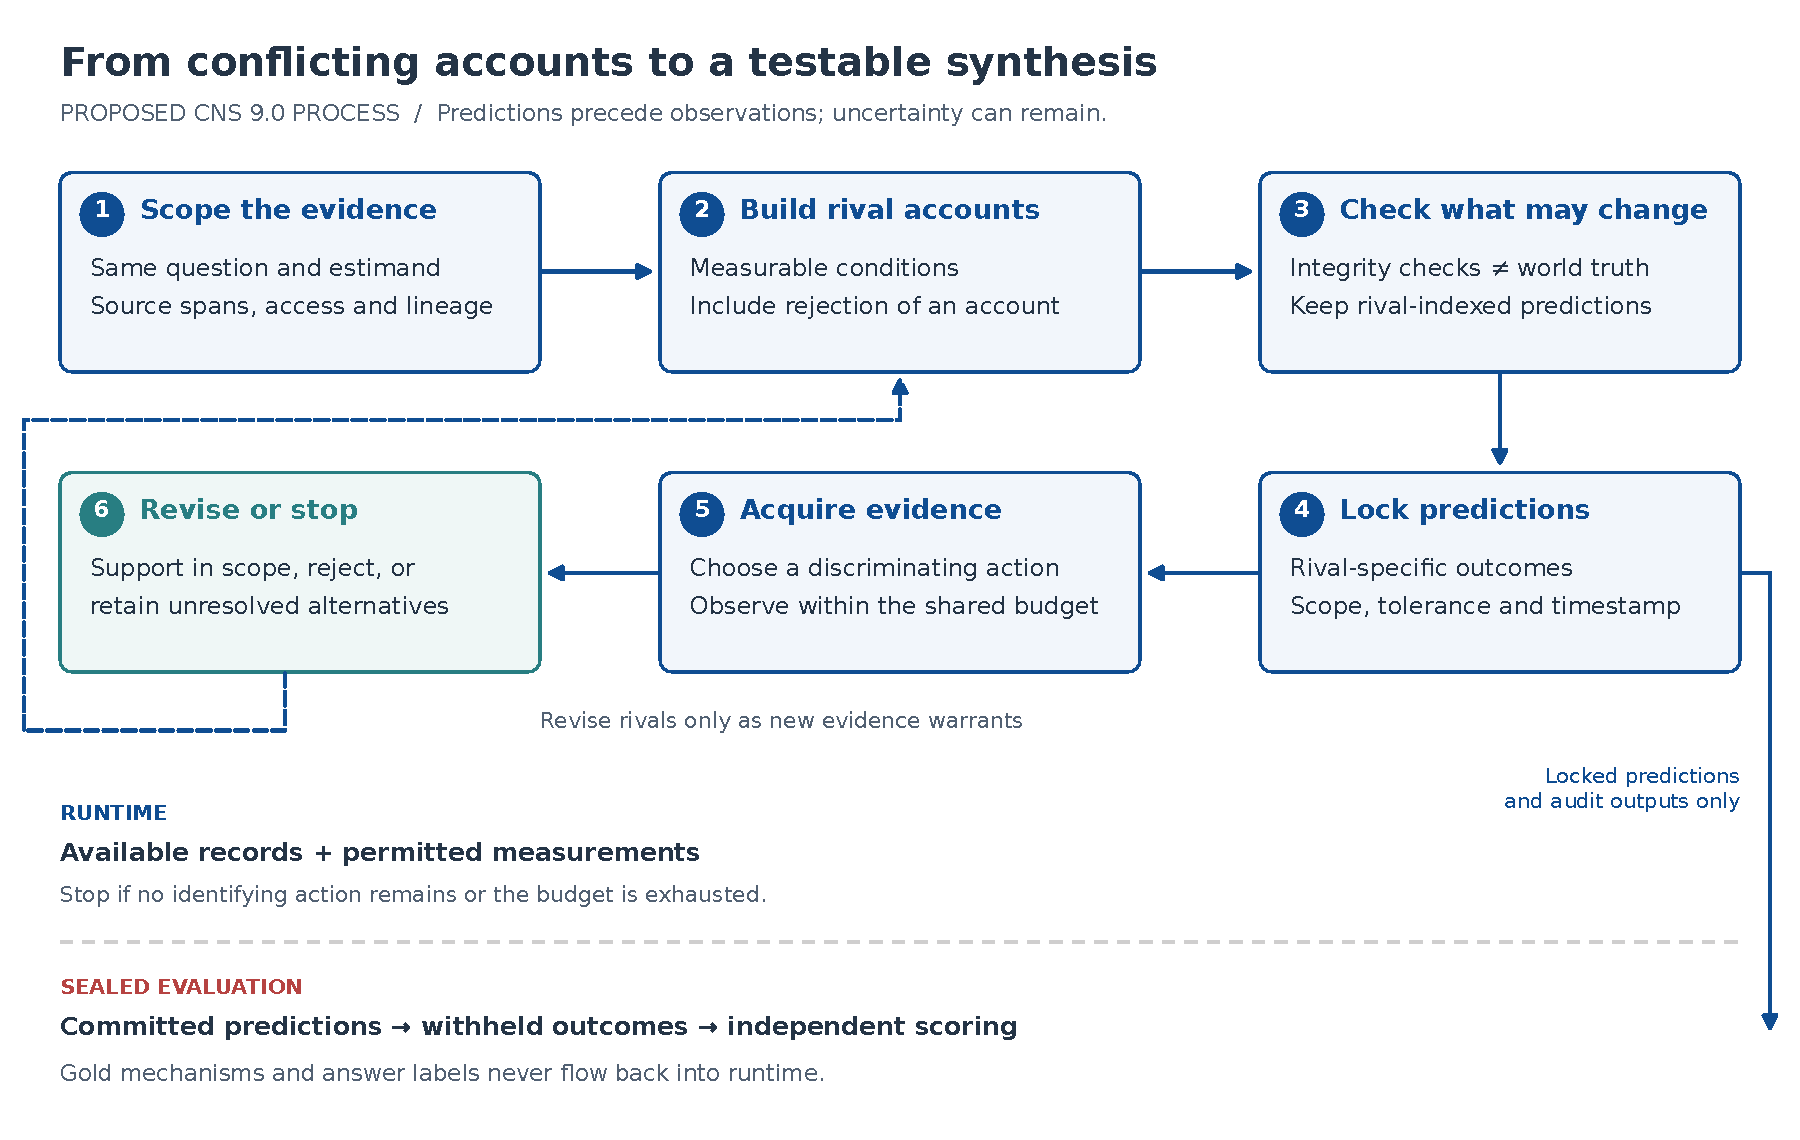
\includegraphics[width=\linewidth]{figures/cns-9-discovery-loop.pdf}
\caption{Proposed discovery loop. Integrity checks and rival-indexed predictions precede acquisition. Only committed outputs cross into sealed evaluation; no gold outcomes return to runtime.}
\label{fig:cns-9-discovery-loop}
\end{figure}

\par\medskip
\noindent\begin{minipage}{\linewidth}
\begin{CNSAlgorithm}
INPUT: scoped question q, permitted evidence E, action menu A,
       model and measurement budgets B
1  Snapshot E; verify spans, units, timestamps and origin lineages.
2  Construct SNO 9 claims and identify same-estimand disagreements.
3  Generate bounded rivals, including rejection and unresolved cases.
4  Separate integrity contracts from rival-indexed response predictions.
5  Validate preconditions; retain unknown contract states.
6  Test contrastive outputs without evaluator labels.
7  Propose bounded, observable scope rules; reject circular rules.
8  Lock novel, distinguishing predictions before new observations.
9  Score feasible actions; observe a permitted separating measurement.
10 Check adequacy; record failures and all-candidates-inadequate states.
11 Repeat within explicit caps, or stop with residual alternatives.
OUTPUT: warranted scoped assertions, locked predictions and audit.
\end{CNSAlgorithm}
\end{minipage}\par\medskip

A contract should not be validated by the same example whose result it
was invented to rationalize. Development can refine the grammar and
validator; calibration can tune abstention; confirmatory cases must be
new. The system may request a measurement from an outcome service, but
that service must return an ordinary reading rather than a hidden label
such as ``hypothesis true.'' The benchmark evaluator sees sealed
mechanisms and withheld predictions \textbf{only after} the runtime
outputs have been committed \citep{G08}.

Validation should be adversarial. A candidate that says ``the cache
helps exactly when it helps'' is circular. A rule invented solely to
rescue every negative example is disallowed by bounded grammar and
held-out tests. A stable false answer fails external correctness. A
continually abstaining system fails coverage. A model that always
reconciles fails on direct-rejection controls. Conversely, a model that
refuses to synthesize whenever sources disagree should fail
discovery-eligible cases. These negative cases are not peripheral; they
determine whether the proposed contribution is real.

\section{Worked example: caching, mechanisms and
refutation}\label{worked-example-caching-mechanisms-and-refutation}

\begin{figure}[htbp]
\centering
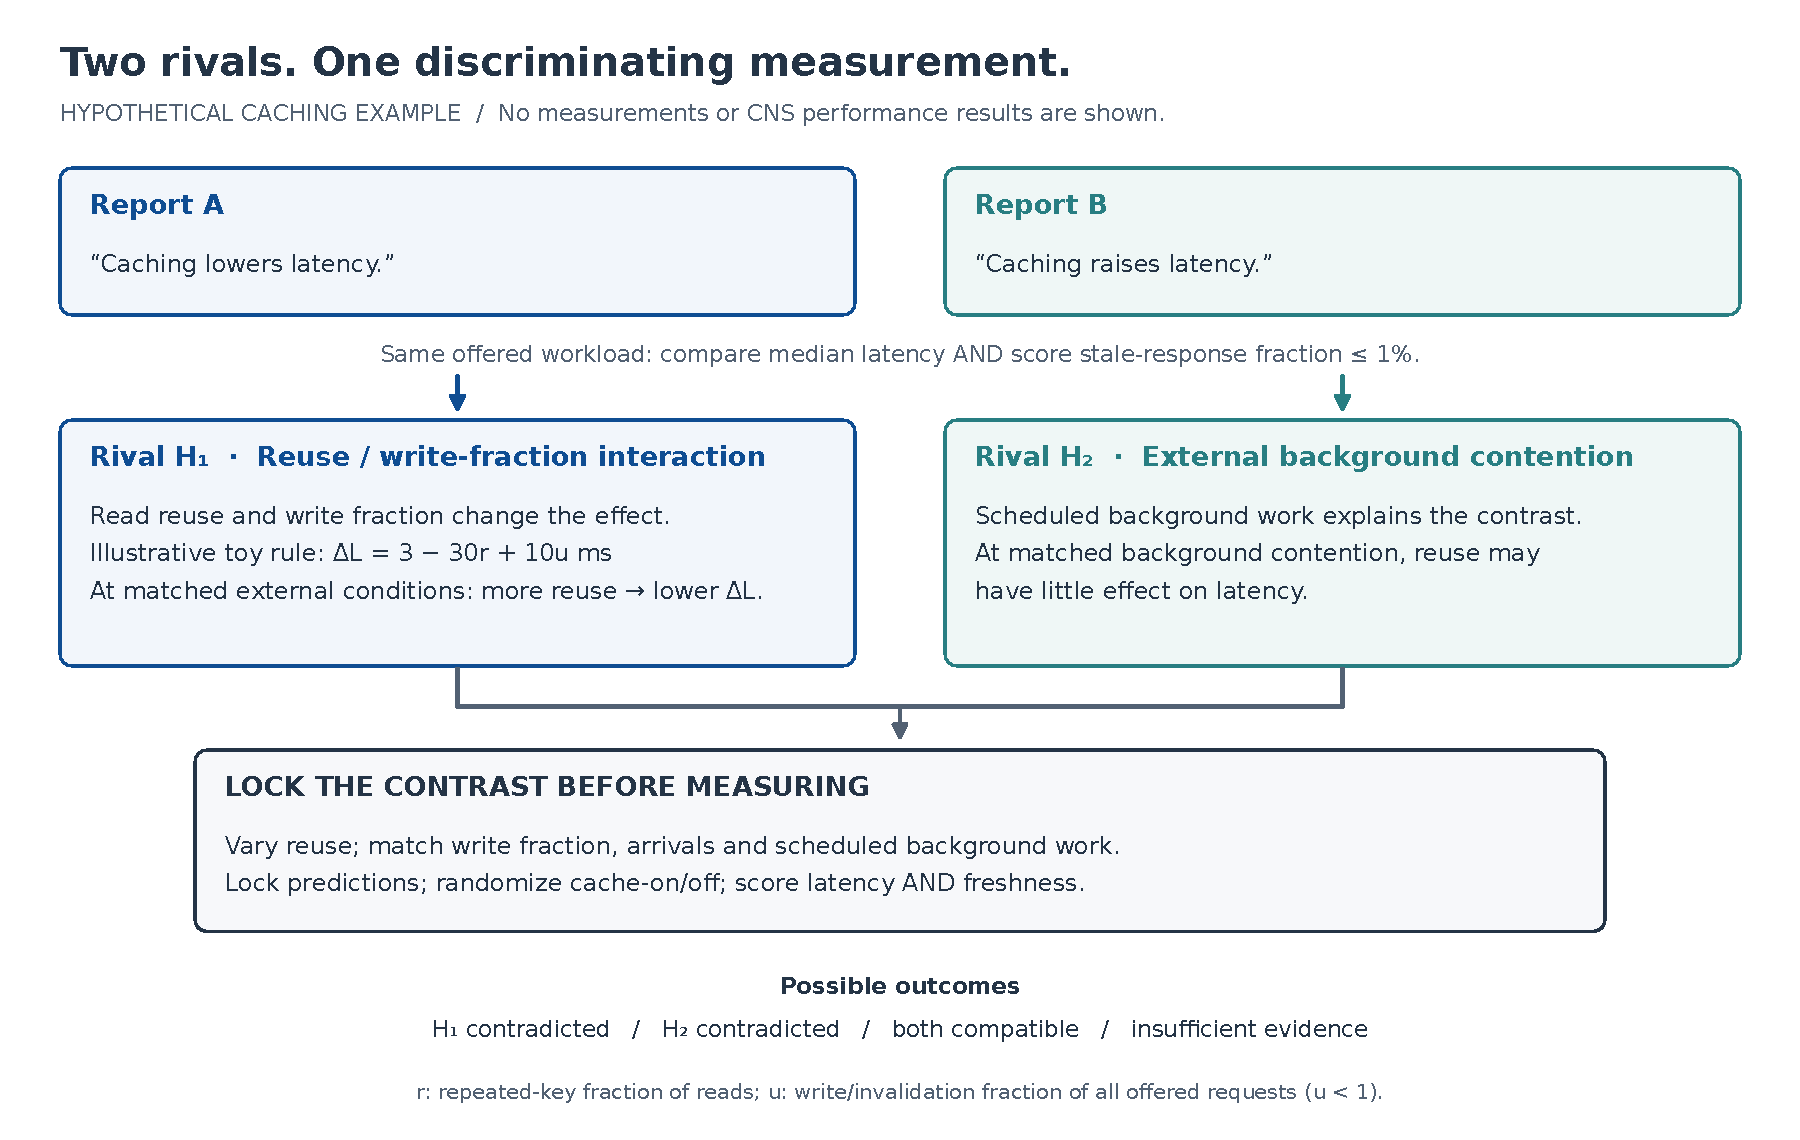
\includegraphics[width=\linewidth]{figures/cns-9-caching-example.pdf}
\caption{Hypothetical caching contrast. Reuse/write-fraction and external-contention rivals commit predictions before a separating measurement. Downstream utilization is not held fixed; latency and freshness are both scored.}
\label{fig:cns-9-caching-example}
\end{figure}

Figure 2 is a \emph{hypothetical illustration}, not a CNS run. Define
\(\Delta L=L_{\mathrm{cache\ on}}-L_{\mathrm{cache\ off}}\) in
milliseconds for a fixed offered workload. Negative values indicate
lower median latency. Separately predict and measure staleness; a
workload is a deployment-success case only if its declared freshness
bound (for example, stale-response fraction at most 0.01) is satisfied.
Do not drop freshness failures after seeing them or condition the
latency estimate on selected successful requests.

Let \(r\) be the fraction of \textbf{read requests} repeating a key
already requested within a prespecified reuse window, and \(u\) the
fraction of \textbf{all offered requests} that are writes/invalidation
requests. Both are dimensionless workload settings, not an observed
cache-hit rate or writes per second. The denominator of \(r\) requires
\(u<1\); feasible key schedules, arrival rate and request mix must be
specified. A relation for communication only is

\[
\Delta L_{\mathrm{toy}}=(3-30r+10u)\ \mathrm{ms},\qquad 0\le r\le1,\quad0\le u<1.
\]

This invented rule is \textbf{not fitted data or a claimed cache
mechanism}. Two reports do not identify its coefficients. Rival \(H_1\)
proposes a reuse/write-fraction interaction. Rival \(H_2\) proposes that
\textbf{externally scheduled background contention} explains the
contrast. External offered traffic and background work can be
controlled; backend utilization caused by cache hits is a mediator, not
a quantity to match across treatment arms. Concurrency policy, hardware
capacity, payload distribution and reuse-window definition must also be
fixed or explicitly varied.

Before observing a new workload, lock each rival's latency and freshness
predictions. A feasible contrast varies reuse while matching write
fraction, offered arrival rate and scheduled background contention; a
complementary contrast varies external contention at matched workload
settings. Randomize cache-on/off order and monitor carryover. Do not
artificially hold downstream CPU/database work constant while claiming
the total caching effect. If neither contrast separates the rivals,
record that limitation. If all candidates fail noise-aware adequacy
checks, reopen within budget or remain model-inadequate.

The prospective evaluator scores commitments against withheld
measurements collected later. Runtime may receive only the outcomes of
permitted acquisition actions, not gold mechanisms or evaluation
verdicts. The same extracted measurements must be available to direct
rule/regression learners. Correct predictive scope need not identify a
unique causal graph; causal wording requires defensible interventions
and assumptions.

\section{Three falsifiable
hypotheses}\label{three-falsifiable-hypotheses}

The following are \textbf{proposed} hypotheses, sample sizes and
ambitious improvement targets. They are not measured effects or a
registered protocol. The full public specification is at
\href{https://gtcode.com/guides/cns-9/evaluation/}{the CNS 9.0 proposed
evaluation page}.

\textbf{H1 --- Contrastive reliability.} Compared with the best
compliant development-selected baseline, will CNS 9.0 more often issue
warranted answers that preserve semantics under six nuisance changes and
respond correctly to four relevant changes? The independent root-level
endpoint requires correct base content and all ten appropriate branch
relations. The proposed primary population has \(n=2400\) roots and an
ambitious target of \textbf{+5 percentage points} in root-level success.
A safeguard on 1,800 resolvable cases demands that the lower one-sided
95\% confidence bound for the coverage difference exceed \textbf{-2
percentage points}. A positive result explained entirely by abstention
would not support H1.

\textbf{H2 --- Independently predictive synthesis.} On 1,200
discovery-eligible roots, will CNS more often generate a measurable,
non-circular scope rule, at least one new distinguishing prediction
absent from the initial narratives, and \textbf{at least four correct
outcomes out of five withheld predictions}? The target is \textbf{+10
percentage points} versus a development-selected comparator pool that
must include the common-extractor learner and iterative refinement
system. On the other 1,200 roots, the upper one-sided 95\% confidence
bound for false novel-scope promotion must not exceed \textbf{5\%}. If a
direct rule learner, regression model, or better-calibrated verifier
matches CNS, the distinctive synthesis hypothesis is weakened or
falsified. H2 is the program's strategic centerpiece.

\textbf{H3 --- Disagreement-guided investigation.} Given the same
reduced evidence and at most \textbf{three external actions / 12 cost
units}, will CNS more often reach the correct scoped conclusion on 1,800
action-resolvable roots than random, relevance-based, uncertainty-only,
or further-discussion alternatives? The target is \textbf{+10 percentage
points}. A 600-root non-identifiable control imposes an upper one-sided
95\% bound of \textbf{5\%} on false resolution. A secondary action-cost
target is 25\% reduction at matched accuracy; it cannot replace a failed
primary endpoint.

The hypotheses may succeed or fail separately. H1 without H2 would
support a contrastive verifier rather than a new method of knowledge
discovery. H3 without H2 could indicate useful active learning based on
ordinary hypotheses. H2 without credible source tracing and withheld
evaluation would not establish the claim being made here. No decision is
rescued by post hoc reweighting of the three endpoints.

\section{Proposed evaluation design and
safeguards}\label{proposed-evaluation-design-and-safeguards}

The controlled study is built around \textbf{independent root worlds},
not the number of prompts. It proposes 120 engineering fixtures outside
the scientific evidence; 600 development roots; 600 calibration roots;
240 pilot roots; and 2,400 confirmatory roots, totaling \textbf{3,840
new research roots}. Confirmatory cases span eight mechanism families
with 300 roots each: confounding; effect modification; selection and
missingness; measurement/representation; regime change; dependent
reporting; rare/nonlinear interactions; and observational equivalence.
F7 and F8 are held out from prompt and generator tuning as families,
with the limitation that pre-trained models may still know the abstract
concepts. The provisional allocation is 150 discovery-eligible, 75
direct/rejection and 75 non-identifiable roots per family (1,200/600/600
overall). These are planning targets pending a target/view feasibility
audit. For F8, causal graphs can remain observationally equivalent while
agreeing on the observational prediction scored by H2; that does not
license causal identification. A root is non-identifiable only if
accessible evidence/actions leave different answers to its declared
target possible. Static and reduced adaptive views are certified
separately. If the proposed cells cannot be constructed without
shortcuts, revise the allocation, denominators and dependent arithmetic
before registration rather than forcing the uniform grid.

Each root supplies one base presentation, six nuisance branches and four
relevant-change branches: \textbf{11 static presentations per root}. An
adaptive action branch starts from a fresh state and may reveal
permitted measurements; it is separate from the static evaluations.
Repeated branches, different prompt orderings and model seeds do not
create additional independent worlds. Gold transformations are
established by generator checks and independent review before the test.
Invalid contracts discovered later are disclosed, not silently removed.

Ten systems are proposed: strong retrieval-augmented generation (B1);
RAG plus chain-of-verification (B2); RAG with self-consistency (B3); an
operational interpretation of the focal essay's multi-context sketch
(B4); a grounded/provenance-aware extension of that sketch (B5);
grounded debate (B6); a transparently documented operational subset of
CNS 8.0 (B7); a common-extractor ordinary learner (B8); a documented
iterative hypothesis-refinement adaptation (B9); and CNS 9.0 (C9). B4
and B5 are \textbf{our documented operationalizations} of Lopez-Paz's
inference-time sketch, not implementations provided by its author. They
do not represent an exhaustive implementation of the essay's broader
philosophical program. Comparisons against them assess these particular
procedures under the stated budgets. B7 must list omissions and cannot
stand for all possible CNS 8.0 systems. B8 and B9 are required primary
H2 comparator candidates. The B8 mechanism comparison shares a fixed
pre-action extraction result and charges extraction to every system;
end-to-end results are also reported. New features invented later are
logged as a separate contribution. B9 uses the same evidence and budget,
with its adaptation to this task disclosed \citep{R37, R38}. Seven
ablations remain secondary controls, alongside matched-information
generic-versus-contradiction-guided candidate generation.
Noncontradictory controls must not remove relevant facts merely to
weaken the alternative.

Fairness requires identical accessible evidence, action menus and
effective compute ceilings, not identical rhetoric or forced token
spending. The proposed budget is at most 120,000 input and 30,000 output
tokens per system-root: eleven static branches at 8,000/2,000 apiece,
and one adaptive branch at 32,000/8,000. Each system has at most three
adaptive actions costing at most 12 units. The primary comparator for
each hypothesis is selected using \textbf{development data only} and
frozen before final evaluation. Two model families and two seeds are
suggested as replications; a prespecified one-family/one-seed
configuration anchors the primary comparisons, and repeated roots are
analyzed as clusters.

The proposal allocates a familywise alpha of 0.05 across three primary
comparisons (Bonferroni, two-sided \(\alpha=0.05/3\)), paired root-level
exact McNemar tests, and \textbf{98.333\%} effect intervals estimated by
a frozen paired bootstrap; a paired-score interval is sensitivity
analysis. Primary claims require both the adjusted exact test and the
frozen bootstrap lower bound to support a positive effect, plus their
safeguards; a test/interval disagreement is reported as inconclusive,
not resolved by choosing the favorable result; reaching a point target
is descriptive unless its adjusted lower confidence bound also exceeds
that target. Absolute 5\% false-promotion/false-resolution limits are
retained, not relaxed to match a weak baseline; their interval method
and attainability under the actual sampling design must be frozen. H1
keeps one strict primary endpoint with required unconditional component
diagnostics; any non-degradation margins are pending. H2 challenge sets
must distinguish plausible rivals by task, not impose sign reversals on
every family. H3 requires sufficient acquired evidence for its target,
not merely a lucky correct guess or a prescribed action. Menus and costs
must be checked for hidden-answer cues. Approximate power calculations
assume a particular discordance rate and are \textbf{not} guarantees of
statistical power. All numeric choices remain changeable \textbf{before}
registration, with a visible versioned amendment history; they may not
change after viewing confirmatory outcomes without breaking the primary
claim.

Transfer tests are proposed, not executed: 900 source-clustered groups
across FEVER, SciFact and AVeriTeC; 60 eligible DiscoveryBench tasks;
and 240 prospective caching/workload scenarios. The caching design calls
for 12 settings per scenario, two cache conditions and three repeats,
yielding \textbf{17,280 planned executions}. Measurements for five
withheld settings would be collected after predictions are locked.
Benchmark labels about document support, fact checking and inferred data
relationships are not interchangeable certificates of external truth.
All study phases require secure runtime/evaluator separation,
source-cluster splits, prediction hashes, frozen inference settings,
deterministic scoring where possible, and independent review of semantic
edge cases.

A failure analysis is part of the design. Leakage of hidden labels, post
hoc tolerance changes, source duplication across splits, or inability to
reproduce the scorer invalidate a confirmatory claim. Excessive
abstention, arbitrary invented predicates, harms from extra model calls,
or gains achieved only against intentionally weak controls count against
CNS 9.0. The prospective scenario-level estimand is conditional on its
service configuration, with hardware/day/carryover blocks; 240 workloads
are not 240 independent mechanisms. Broader transfer claims require
multiple independently defined regimes and an analysis appropriate to
the number of clusters. A synthetic success without prospective transfer
would support at most a narrower benchmark result, not generalized
scientific discovery. An optional future feasibility study may diagnose
extraction, scoring and acquisition bottlenecks before scaling; no small
fixed effect threshold is claimed decisive and no experiment is
scheduled by this proposal.

\section{Relationship to earlier CNS and design
choices}\label{relationship-to-earlier-cns-and-design-choices}

\begin{figure}[htbp]
\centering
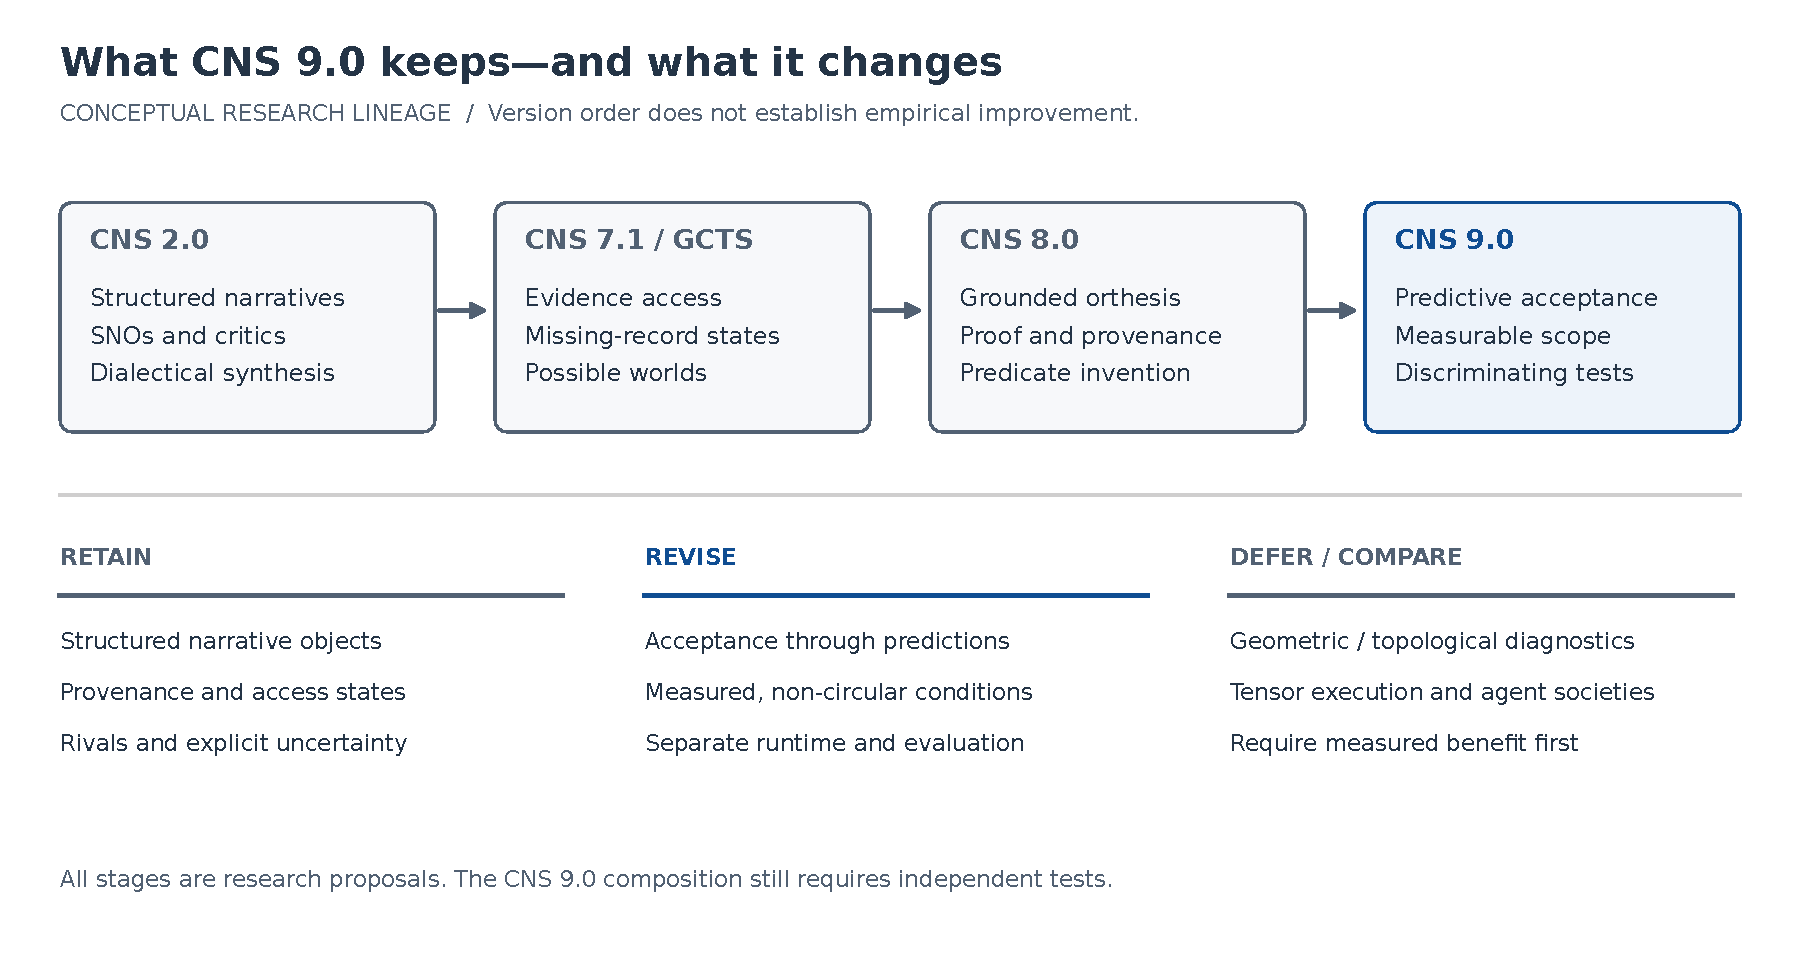
\includegraphics[width=\linewidth]{figures/cns-9-research-lineage.pdf}
\caption{Conceptual research lineage, not measured improvement. CNS 9.0 retains structured evidence and uncertainty while evaluating predictive acceptance against simpler alternatives.}
\label{fig:cns-9-research-lineage}
\end{figure}

Figure 3 depicts conceptual lineage rather than measured improvement.
CNS 2.0 introduced a research program around SNOs, chiral opposition and
criticism; GCTS 7.1 emphasized grounded evidence and access-state
distinctions; CNS 8.0 restored synthesized SNOs and proposed orthesis
conditions, proof traces and bounded predicate invention
\citep{G13, G11, G02, G09}. CNS 8.0 already states that orthesis
stability is not metaphysical truth and can preserve unresolved
contradictions. The 9.0 move is therefore \textbf{a change in scientific
acceptance criteria}, not an assertion that previous versions were
incapable of uncertainty.

The proposal retains structured accounts, provenance, versioned
revisions, rival interpretations, and the ability to construct a
conditional new account. It revises the meaning of productive conflict:
shared target, explicit evidentiary relationships and \textbf{testable
differences in predictions} matter more than a single combined chirality
score. The previous literature's use of ``Evidential Entanglement''
conflated at times shared evidence identifiers with comparable study
endpoints; CNS 9.0 records semantic comparability, shared records and
source copying independently \citep{G09}.

Proof closure remains useful for checking derivability from stipulated
premises. Round-trip language-to-logic fidelity remains useful for
identifying translation errors. Neither becomes a world-truth
certificate. Manifold geometry, curvature, holonomy, topological
reduction, tensor execution and large multiagent societies are
\textbf{optional future comparators}, not prerequisites. They should
return only if a specific reproducible task demonstrates gains beyond
simpler representations at acceptable cost. The original work is
preserved as prior art rather than rewritten as validated implementation
evidence.

\section{Risks, limits, and alternative
explanations}\label{risks-limits-and-alternative-explanations}

\textbf{Admissibility is underspecified in the world.} A model may call
a transformation irrelevant even though it changes the question, or
reject a relevant change because it undermines a preferred answer.
Independently reviewed development contracts and held-out contract
families reduce---but cannot eliminate---this risk. Unknown status is a
real output, not an embarrassment to erase.

\textbf{The hypothesis language introduces bias.} Restricting candidates
to measurable thresholds and simple interactions makes evaluation
possible but could miss a genuine mechanism. Expanding the language
risks overfitting, combinatorial search and post hoc excuses. The
primary study should report both failures to represent the truth and
unjustified inventions; neither can be cured silently after unblinding.

\textbf{Synthetic worlds may reward the generator's assumptions.} A test
set built from the designer's mechanism families can privilege
algorithms that match those families. External tasks, unseen families
and prospectively acquired data must therefore count heavily in
interpretation, even though none establishes universality. Publication
of generator code after evaluation is necessary but not sufficient if
the models' training corpora contain familiar templates.

\textbf{Evidence is not independent just because prose differs.} Copied
records, model-generated perspectives and repeated calls may share the
same error. The dependency graph itself can be uncertain. A fair
comparison must give baseline systems the same provenance fields and
assess the ability to detect unknown dependencies rather than scoring a
fabricated certainty.

\textbf{Observation policy can be harmful or uninformative.} High
information gain may target the wrong hypothesis class or exceed a
privacy, safety, or resource budget. The first prospective example is a
sandboxed software service, not human subjects or clinical
interventions. External actions require domain-specific permission and
governance; the proposal confers no authority to run arbitrary
experiments.

\textbf{The explanatory narrative may be unfaithful.} A plausible causal
sentence is not proof of the model's actual inference process
\citep{R18}. The deliverable should be a compact, source-linked and
checkable claim, its prediction record and its test outcome. Causal
language should be reserved for designs where the identification
assumptions are defensible.

\textbf{Alternatives may explain any future gain.} A structured SNO
schema, more compute, a better retrieval index, source deduplication,
direct regression, or simpler active learning could capture all apparent
improvement. The proposed ablations and well-resourced baseline suite
are not optional ornaments; they make the theory vulnerable to
disconfirmation.

\textbf{The ambition is domain-limited.} Scientific and software
observations sometimes admit controlled interventions and clear metrics.
Historical claims, sparse observational science and normative
disagreement may not. CNS must say ``unresolved'' where there is no
permitted identifying observation, rather than imply that every
contradiction hides a discoverable conditional truth.

\section{Research agenda and
conclusion}\label{research-agenda-and-conclusion}

The first scientific gate is not to implement all imagined subsystems.
It is to implement a narrow, auditable slice and a benchmark whose
generator, action service and scorer cannot leak target answers to the
runtime. A second gate tests whether novel scope rules predict hidden
observations better than selection, verification and simple induction. A
third evaluates whether choosing discriminating actions changes what the
system can legitimately conclude. Only after these gates should
training, learned contract discovery, more elaborate geometry or broader
causal claims be considered.

CNS 9.0's ambition is that contradiction can be used as a
\textbf{resource for constructing testable predictive explanations}. The
thesis is narrower than ``truth is invariance,'' yet more demanding than
``multiple agents reach consensus.'' Its value depends on surviving
deliberately adversarial evaluation: when evidence is strong, it should
predict; when evidence refutes a candidate, it should retract; when
independent observations discriminate rivals, it should seek them; and
when the record does not identify an answer, it should stop honestly. A
successful implementation would provide evidence that this particular
composition has value on stated classes of problems. A failure should
simplify the architecture or retire the claim, not motivate additional
untested mathematical decoration.

\section{Citation and version note}\label{citation-and-version-note}

\textbf{GTCode.com (15 November 2026).} \emph{Chiral Narrative Synthesis
9.0: Falsification-Guided Narrative Synthesis for Predictive Knowledge
Discovery}. Research proposal, version 0.1. Canonical edition:
\textbf{https://gtcode.com/papers/cns-9/}. This version is not peer
reviewed, not preregistered, and contains \textbf{no CNS 9.0
experimental results}. The web research article, the compiled PDF, and
the supplied LaTeX source correspond to the same v0.1 substantive
manuscript. A public companion
\href{https://gtcode.com/guides/cns-9/overview/}{overview} and
\href{https://gtcode.com/guides/cns-9/evaluation/}{proposed evaluation
specification} are separate interpretive and protocol documents.

\bibliographystyle{unsrtnat}
\bibliography{references}
\end{document}
